\documentclass[12pt]{article}
\usepackage[letterpaper,margin=0.75in]{geometry}
\usepackage{xcolor}
\usepackage{fancyhdr}
\usepackage{tgschola} % or any other font package you like
\usepackage{graphicx}
\usepackage{amsmath,amssymb,amsfonts}

\usepackage{titlesec}
\titleformat*{\section}{\large\bfseries}
\titleformat*{\subsection}{\normalsize\bfseries}

% \pagestyle{fancy}
% \fancyhf{}
% \fancyhead[C]{%
%   \footnotesize\sffamily
%   %\yourname\quad
%   Website: \textcolor{blue}{\itshape\yourweb}\quad
%   E-mail: \textcolor{blue}{\youremail}
% }

\newcommand{\soptitle}{Non-autoregressive time-series methods for stable parameteric reduced-order models}
\newcommand{\yourname}{Supporting material}
% \newcommand{\youremail}{romit.maulik@okstate.edu}
% \newcommand{\yourweb}{https://www.cfdlab.org/}

\newcommand{\statement}[1]{\par\medskip
  \underline{\textcolor{blue}{\textbf{#1:}}}\space
}

\usepackage[
  colorlinks,
  breaklinks,
  pdftitle={\yourname - \soptitle},
  pdfauthor={\yourname},
  unicode
]{hyperref}

\begin{document}

\begin{center}
\large
\textbf{
\soptitle} \\
\normalsize
\yourname
\end{center}

\hrule
%\vspace{1pt}
%\hrule height 1pt

\bigskip

\section{The shallow water equations}

Our assessments utilize the inviscid shallow-water equations, which belong to prototypical system of equations for geophysical flows. In particular, the shallow-water equations admit solutions where advection dominates dissipation and poses challenges for conventional model-order reduction methods. The governing equations are hyperbolic in nature and they are given by
\begin{align}
    \frac{\partial(\rho \eta)}{\partial t}+\frac{\partial(\rho \eta u)}{\partial x}+\frac{\partial(\rho \eta v)}{\partial y} =0  \label{eq1} \\
    \frac{\partial(\rho \eta u)}{\partial t}+\frac{\partial}{\partial x}\left(\rho \eta u^{2}+\frac{1}{2} \rho g \eta^{2}\right)+\frac{\partial(\rho \eta u v)}{\partial y} = 0 \label{eq2} \\
    \frac{\partial(\rho \eta v)}{\partial t}+\frac{\partial(\rho \eta u v)}{\partial x}+\frac{\partial}{\partial y}\left(\rho \eta v^{2}+\frac{1}{2} \rho g \eta^{2}\right) = 0, \label{eq3}
\end{align}
where, $\eta$ corresponds to the total fluid column height, and $(u,v)$ is the fluid's horizontal flow velocity, averaged across the vertical column, $g$ is acceleration due to gravity, and $\rho$ is the fluid density, typically set to 1.0. Here, $t,x$ and $y$ are the independent variables time and the spatial coordinates of the two-dimensional system. Equation \ref{eq1} captures the law of mass conservation, whereas Equations \ref{eq2} and \ref{eq3} denote the conservation of momentum. The initial conditions are given by 
\begin{align}
    \rho \eta (x,y,t=0) &= e^{-\left(\frac{(x-\bar{x})^2}{2(5e+4)^2} + \frac{(y-\bar{y})^2}{2(5e+4)^2}\right)} \\
    \rho \eta u(x,y,t=0) &= 0 \\
    \rho \eta v(x,y,t=0) &= 0,
\end{align}
while our two-dimensional domain is a square and utilizes periodic boundary conditions. Our data generation process utilizes full-order solves of the above system of equations until $t=0.5$ with a time step of 0.001. Our full-order model uses a 4\textsuperscript{th}-order accurate Runge-Kutta temporal integration scheme and a fifth-order accurate weighted essentially non-oscillatory scheme (WENO) \cite{liu1994weighted} for computing state reconstructions at cell faces. The Rusanov Reimann solver is utilized for flux reconstruction after cell-face quantities are calculated. We solve these equations using 64 points in each direction to obtain snapshots of our \emph{true} data. We integrate these PDEs in time using a fourth-order accurate in time ODE solver \cite{hairer1991solving}.


\section{Predictions for other PCA coefficients}

In this section, we add results for PCA coefficient predictions for other modes. Note that these can also be retrieved from the supporting code. We show results from the first four modes for results without the incorporation of dropout in Figures \ref{Mode_1}, \ref{Mode_2}, \ref{Mode_3}, \ref{Mode_4}. The trends from from the main article, which show only mode 1, are repeated across different coefficients. The incorporation of dropout in inference lets us assess the long-term robustness to error propagation as seen in Figures \ref{Mode_1_do}, \ref{Mode_2_do}, \ref{Mode_3_do} and \ref{Mode_4_do}. Autoregressive frameworks and their issues with stable long term predictions are once again witnessed.

\begin{figure}[h]
    \centering
    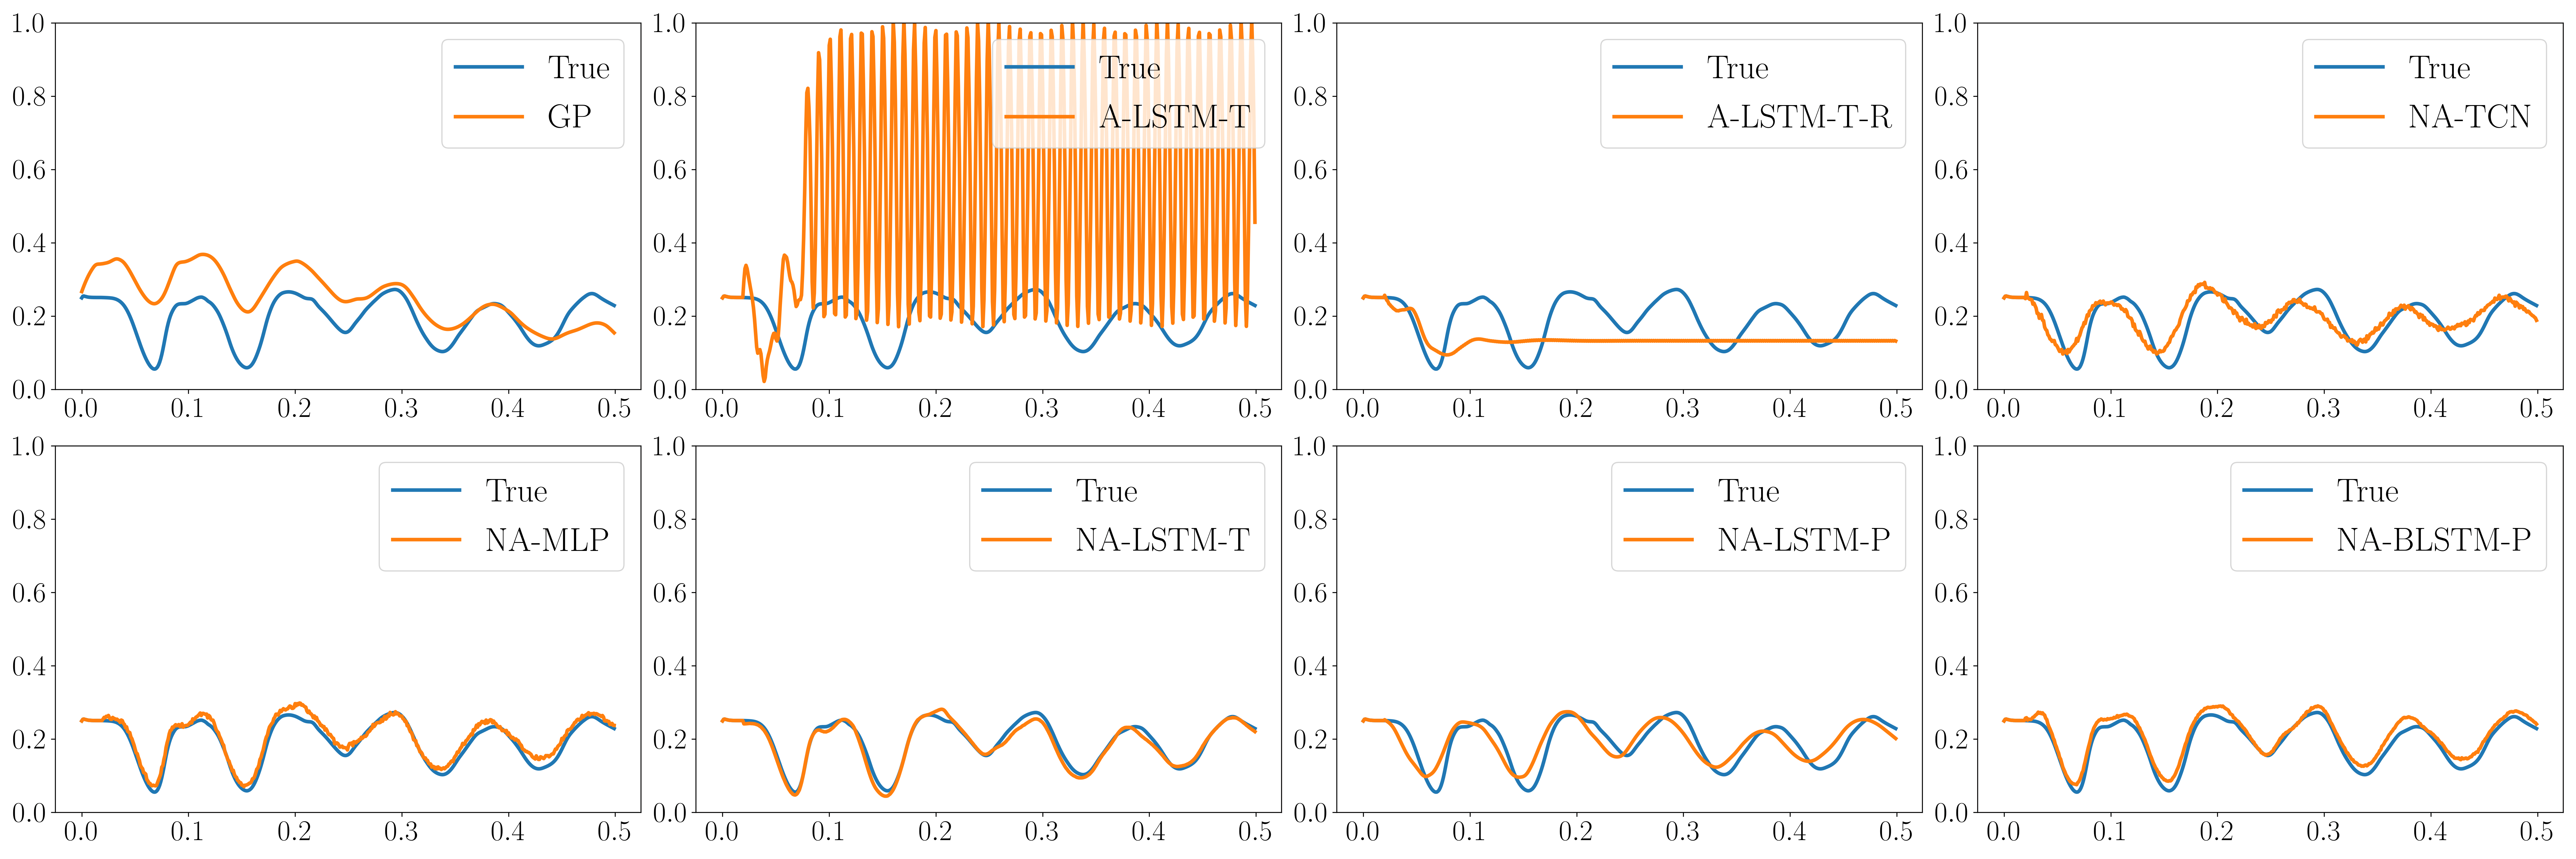
\includegraphics[width=\textwidth]{Figure_1.png}
    \caption{Predictive ability for the assessed frameworks for PCA component 1. We remind the reader that GP requires the solution of a partial differential equation in addition to greater observations from the true system to build a model. In addition, GP is deterministic.}
    \label{Mode_1}
\end{figure}

\begin{figure}[h]
    \centering
    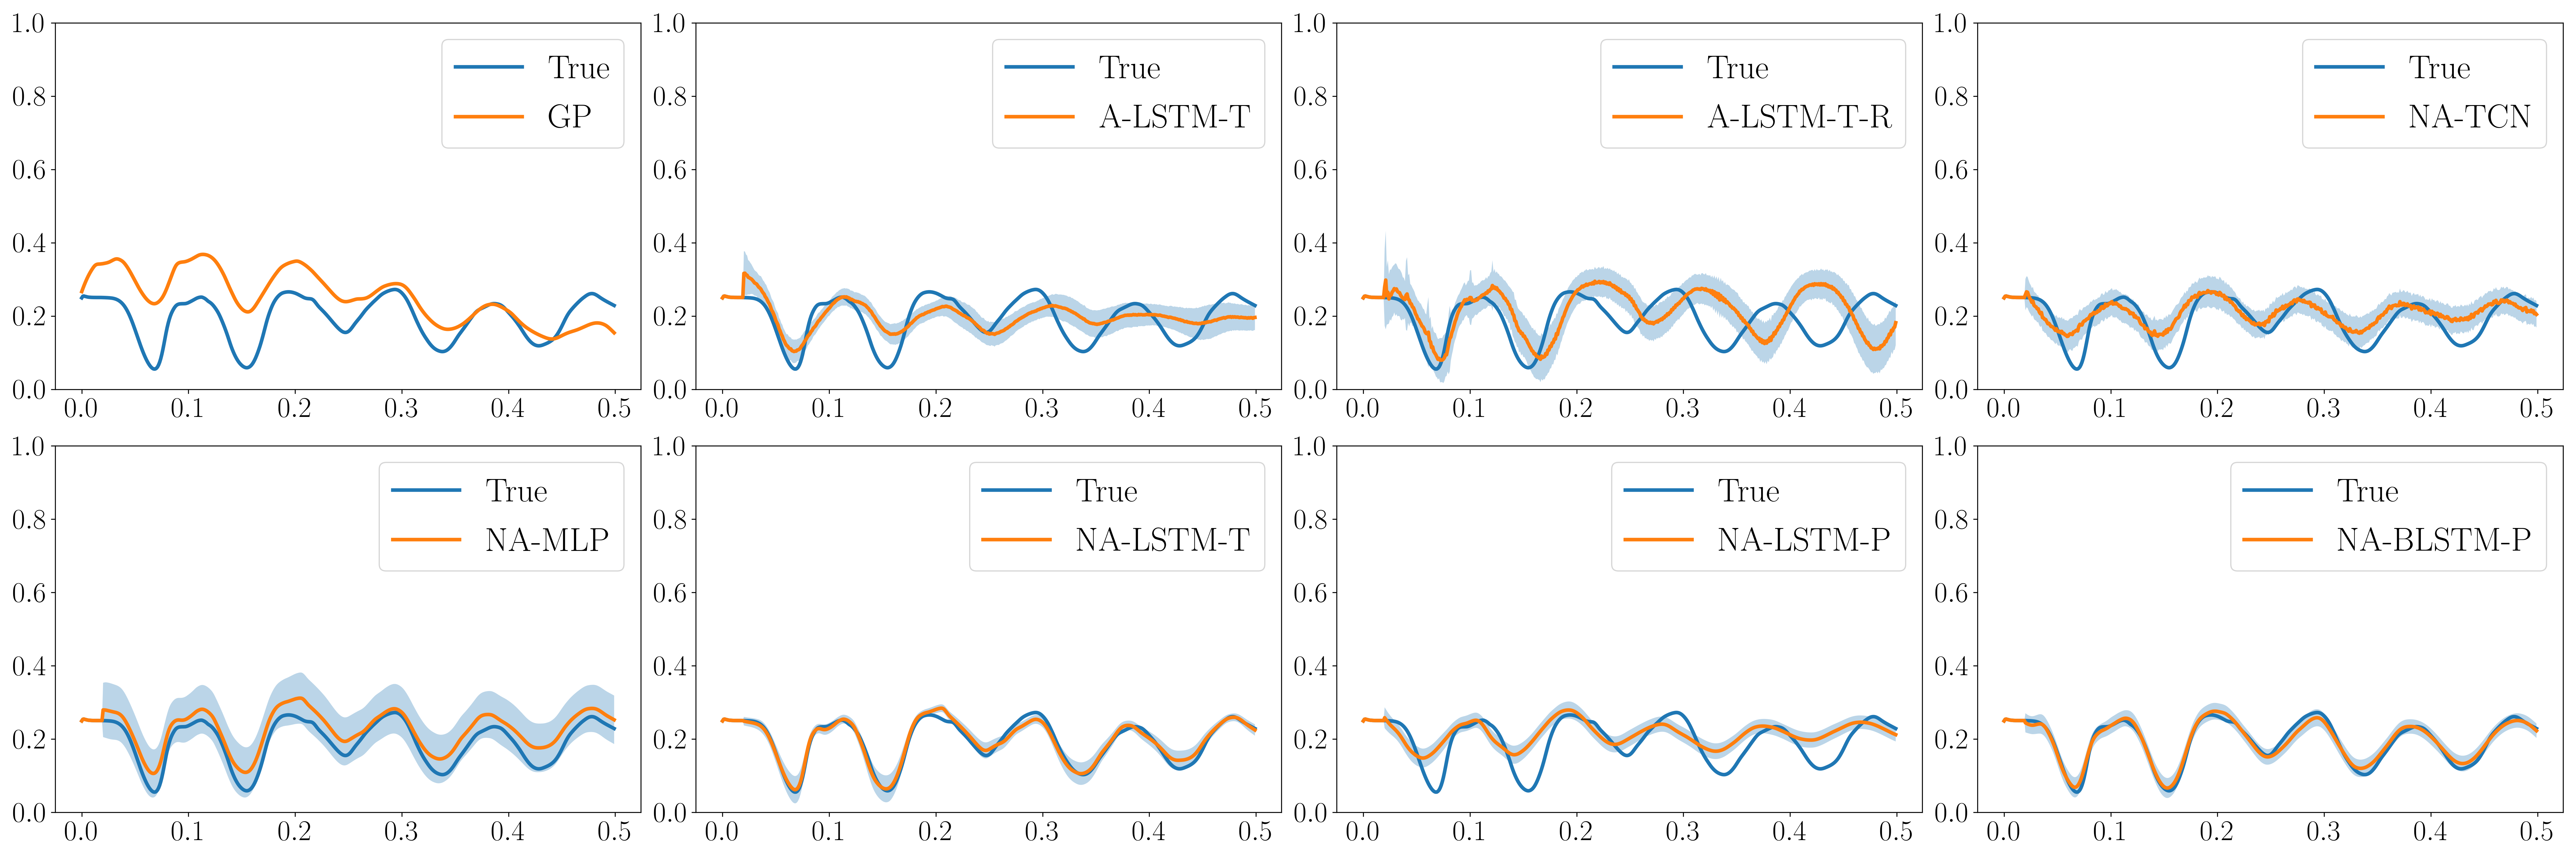
\includegraphics[width=\textwidth]{Figure_1_do.png}
    \caption{Predictive ability for the assessed frameworks for PCA component 1 with dropout at inference. We remind the reader that GP requires the solution of a partial differential equation in addition to greater observations from the true system to build a model. In addition, GP is deterministic.}
    \label{Mode_1_do}
\end{figure}

\begin{figure}[h]
    \centering
    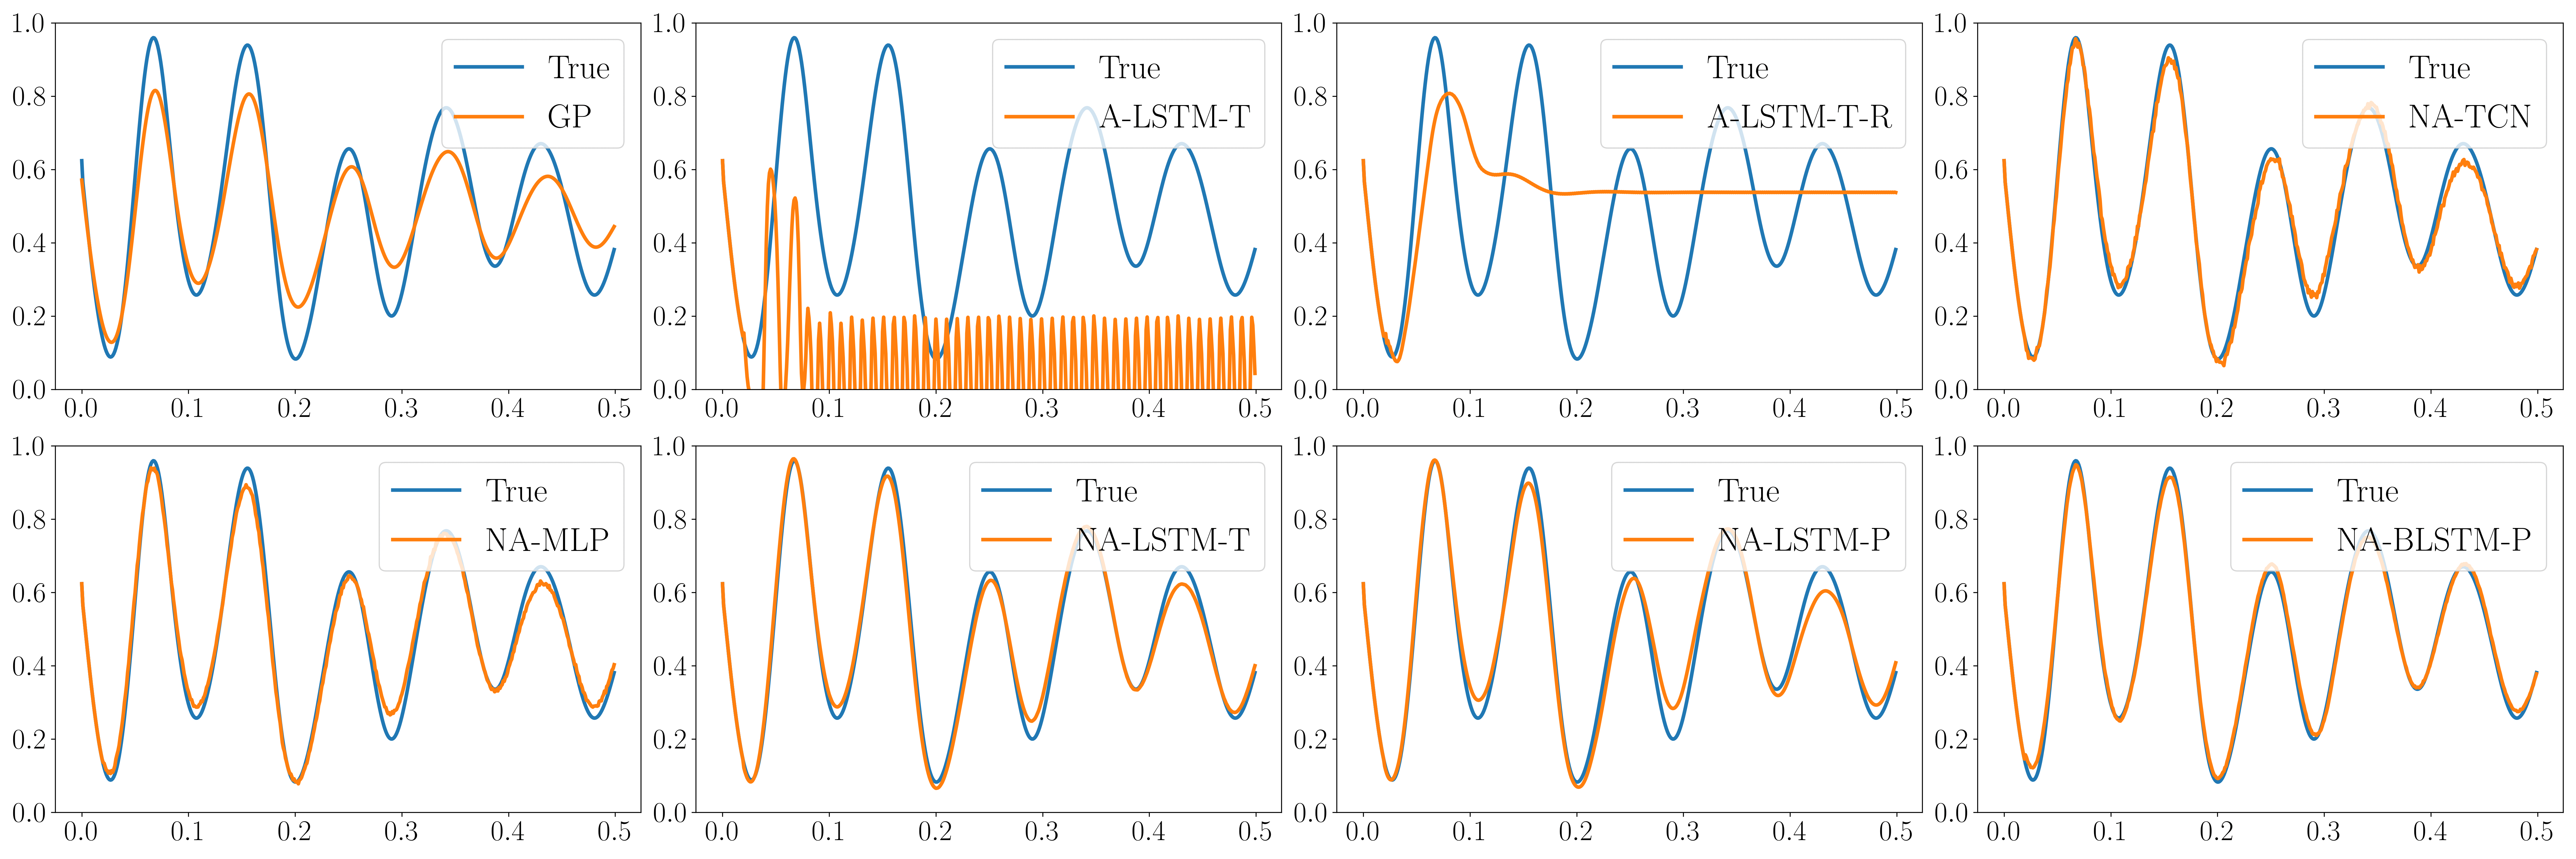
\includegraphics[width=\textwidth]{Figure_2.png}
    \caption{Predictive ability for the assessed frameworks for PCA component 2. We remind the reader that GP requires the solution of a partial differential equation in addition to greater observations from the true system to build a model. In addition, GP is deterministic.}
    \label{Mode_2}
\end{figure}

\begin{figure}[h]
    \centering
    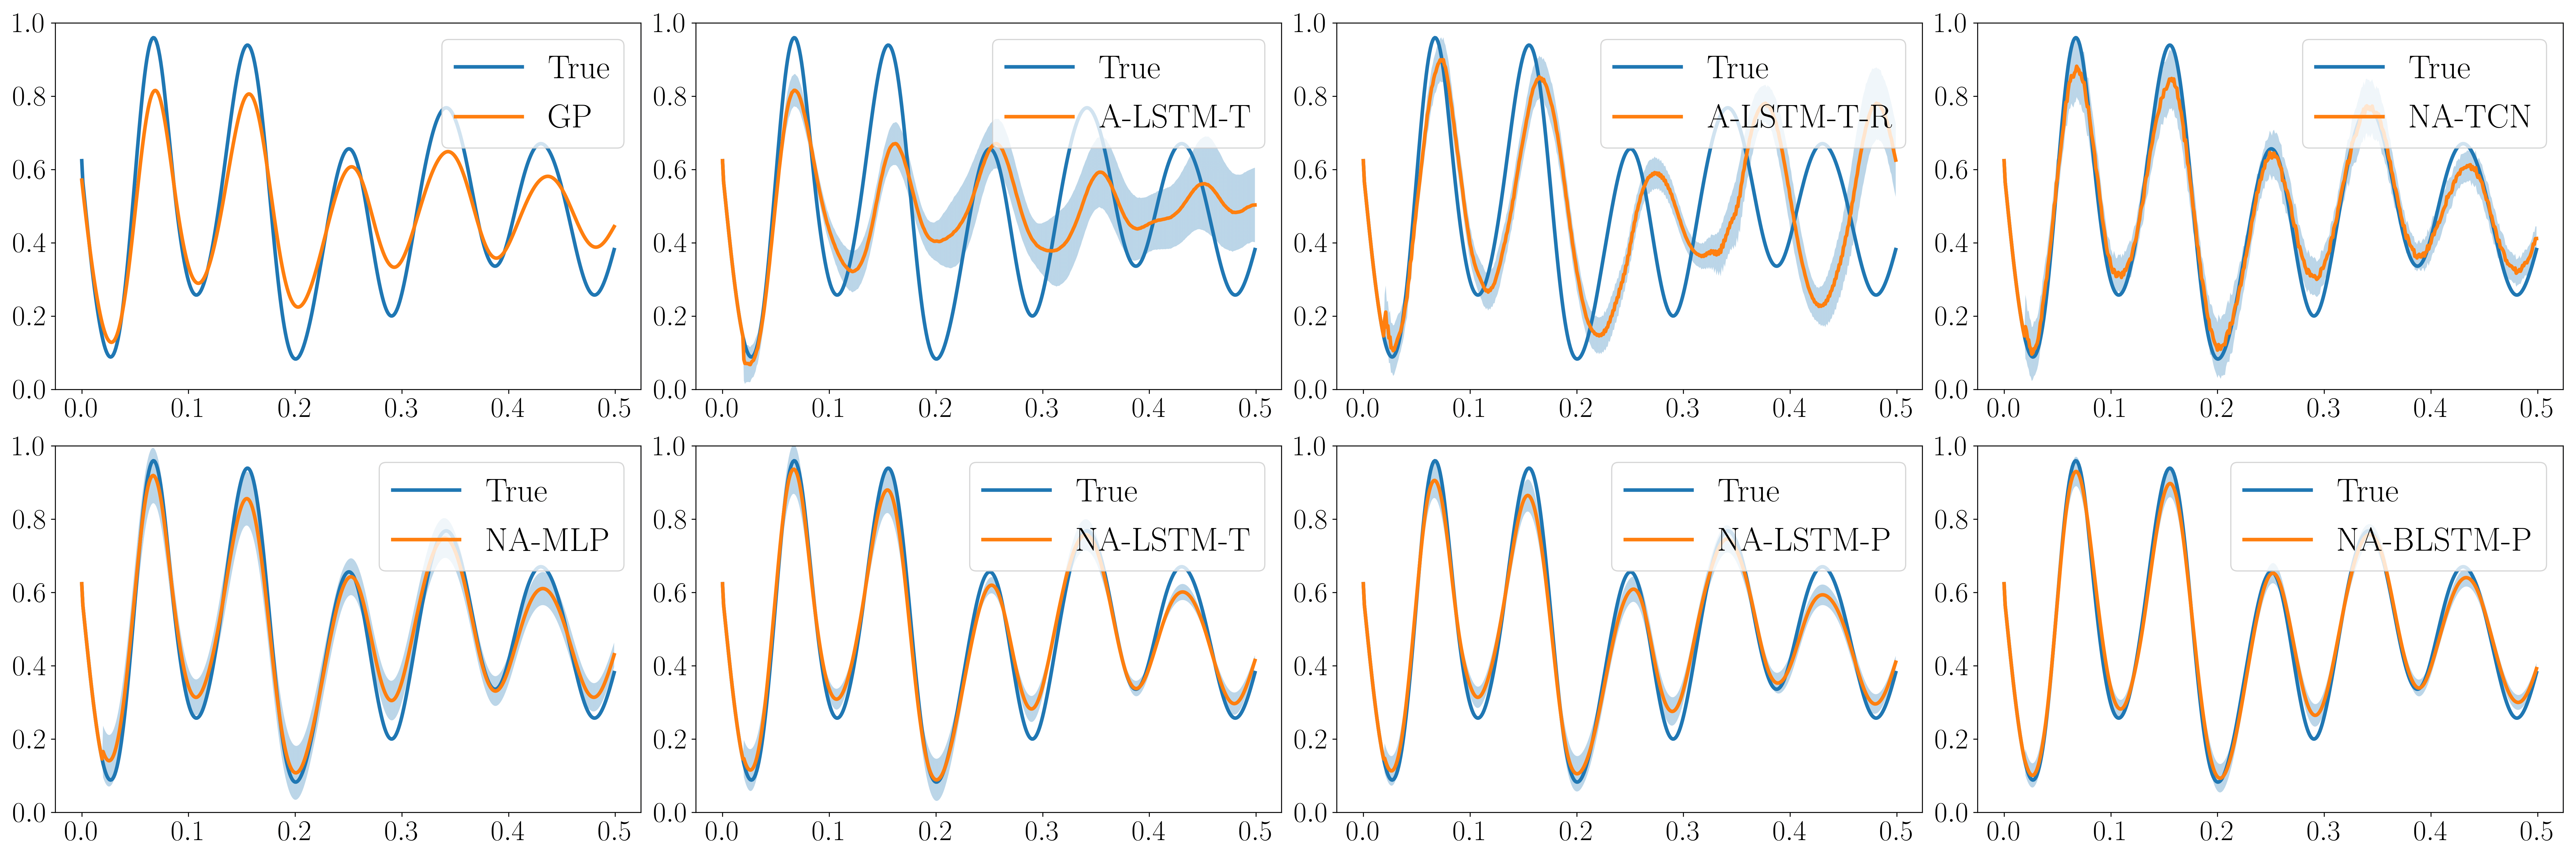
\includegraphics[width=\textwidth]{Figure_2_do.png}
    \caption{Predictive ability for the assessed frameworks for PCA component 2 with dropout at inference. We remind the reader that GP requires the solution of a partial differential equation in addition to greater observations from the true system to build a model. In addition, GP is deterministic.}
    \label{Mode_2_do}
\end{figure}

\begin{figure}[h]
    \centering
    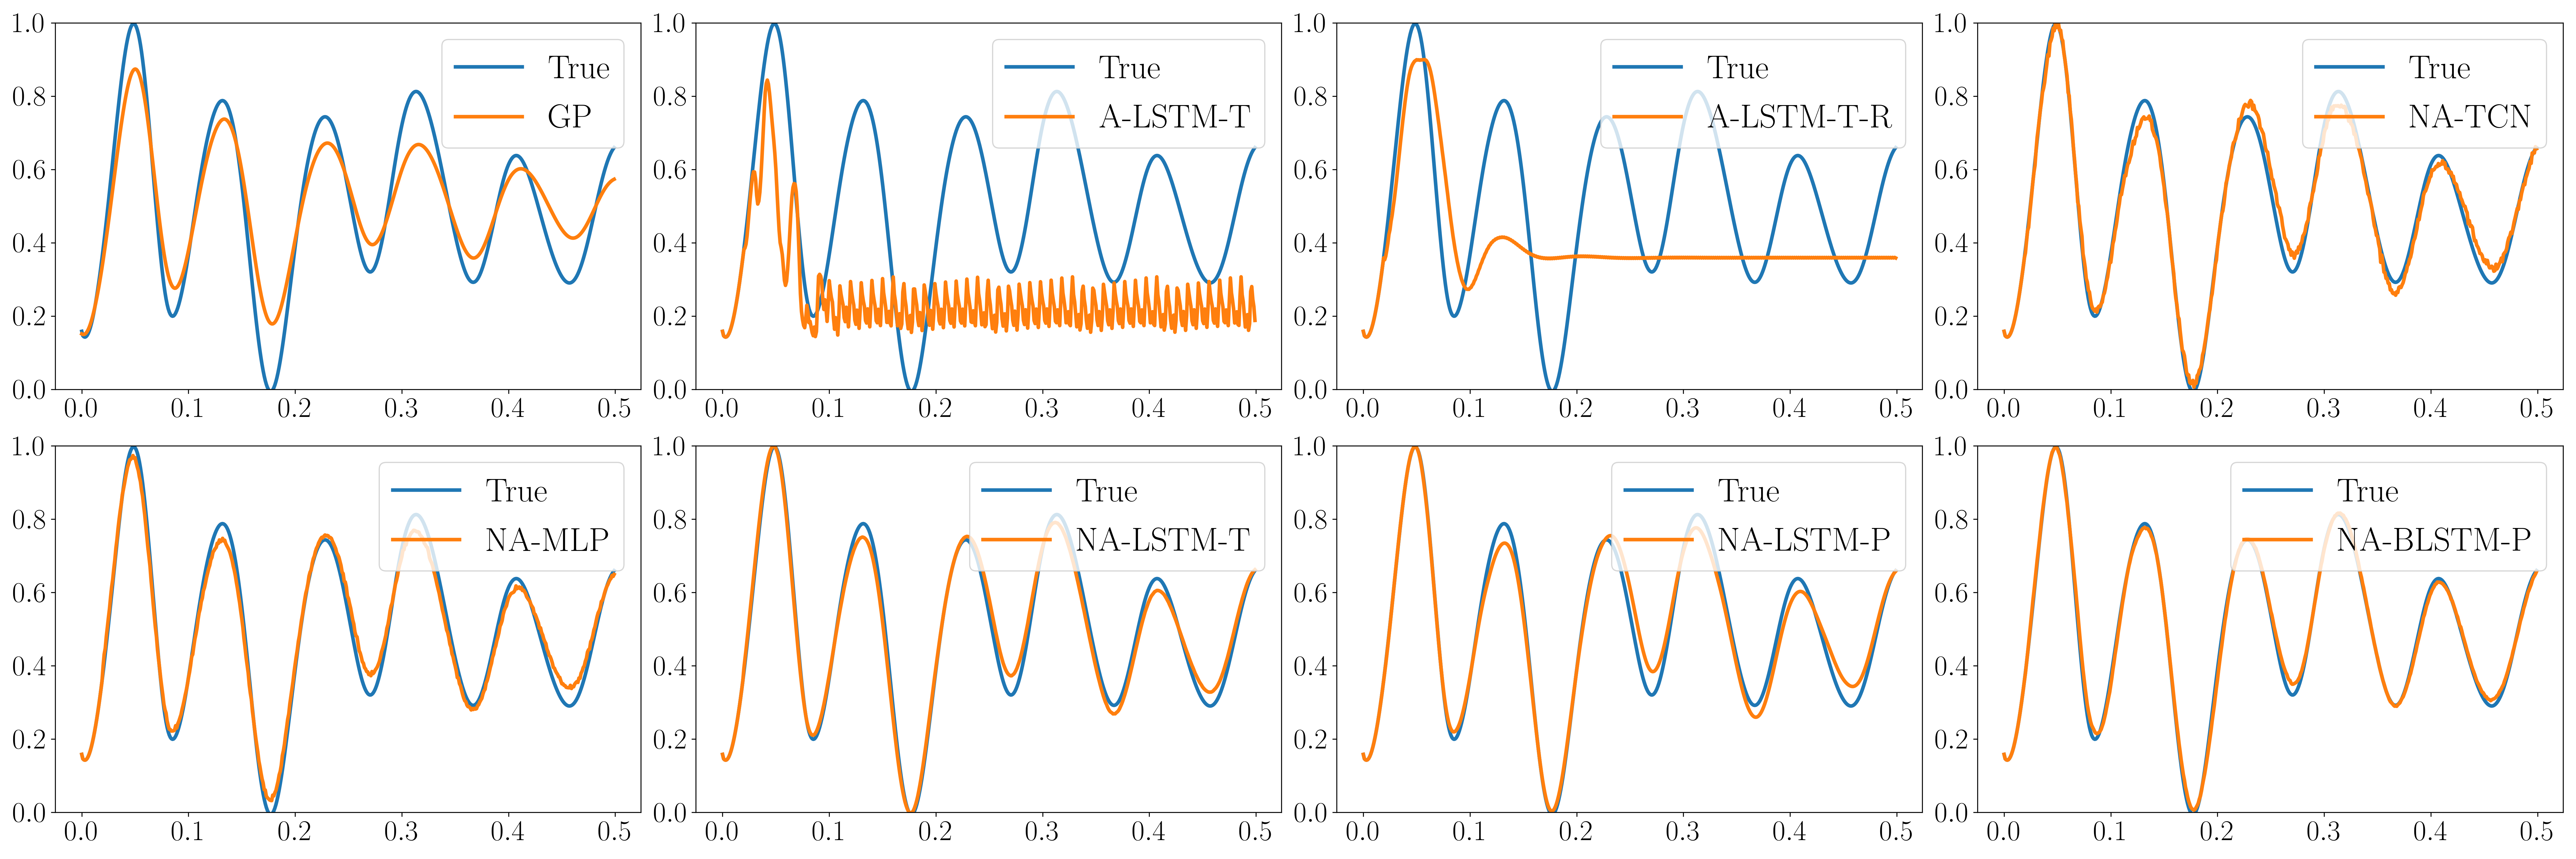
\includegraphics[width=\textwidth]{Figure_3.png}
    \caption{Predictive ability for the assessed frameworks for PCA component 3. We remind the reader that GP requires the solution of a partial differential equation in addition to greater observations from the true system to build a model. In addition, GP is deterministic.}
    \label{Mode_3}
\end{figure}

\begin{figure}[h]
    \centering
    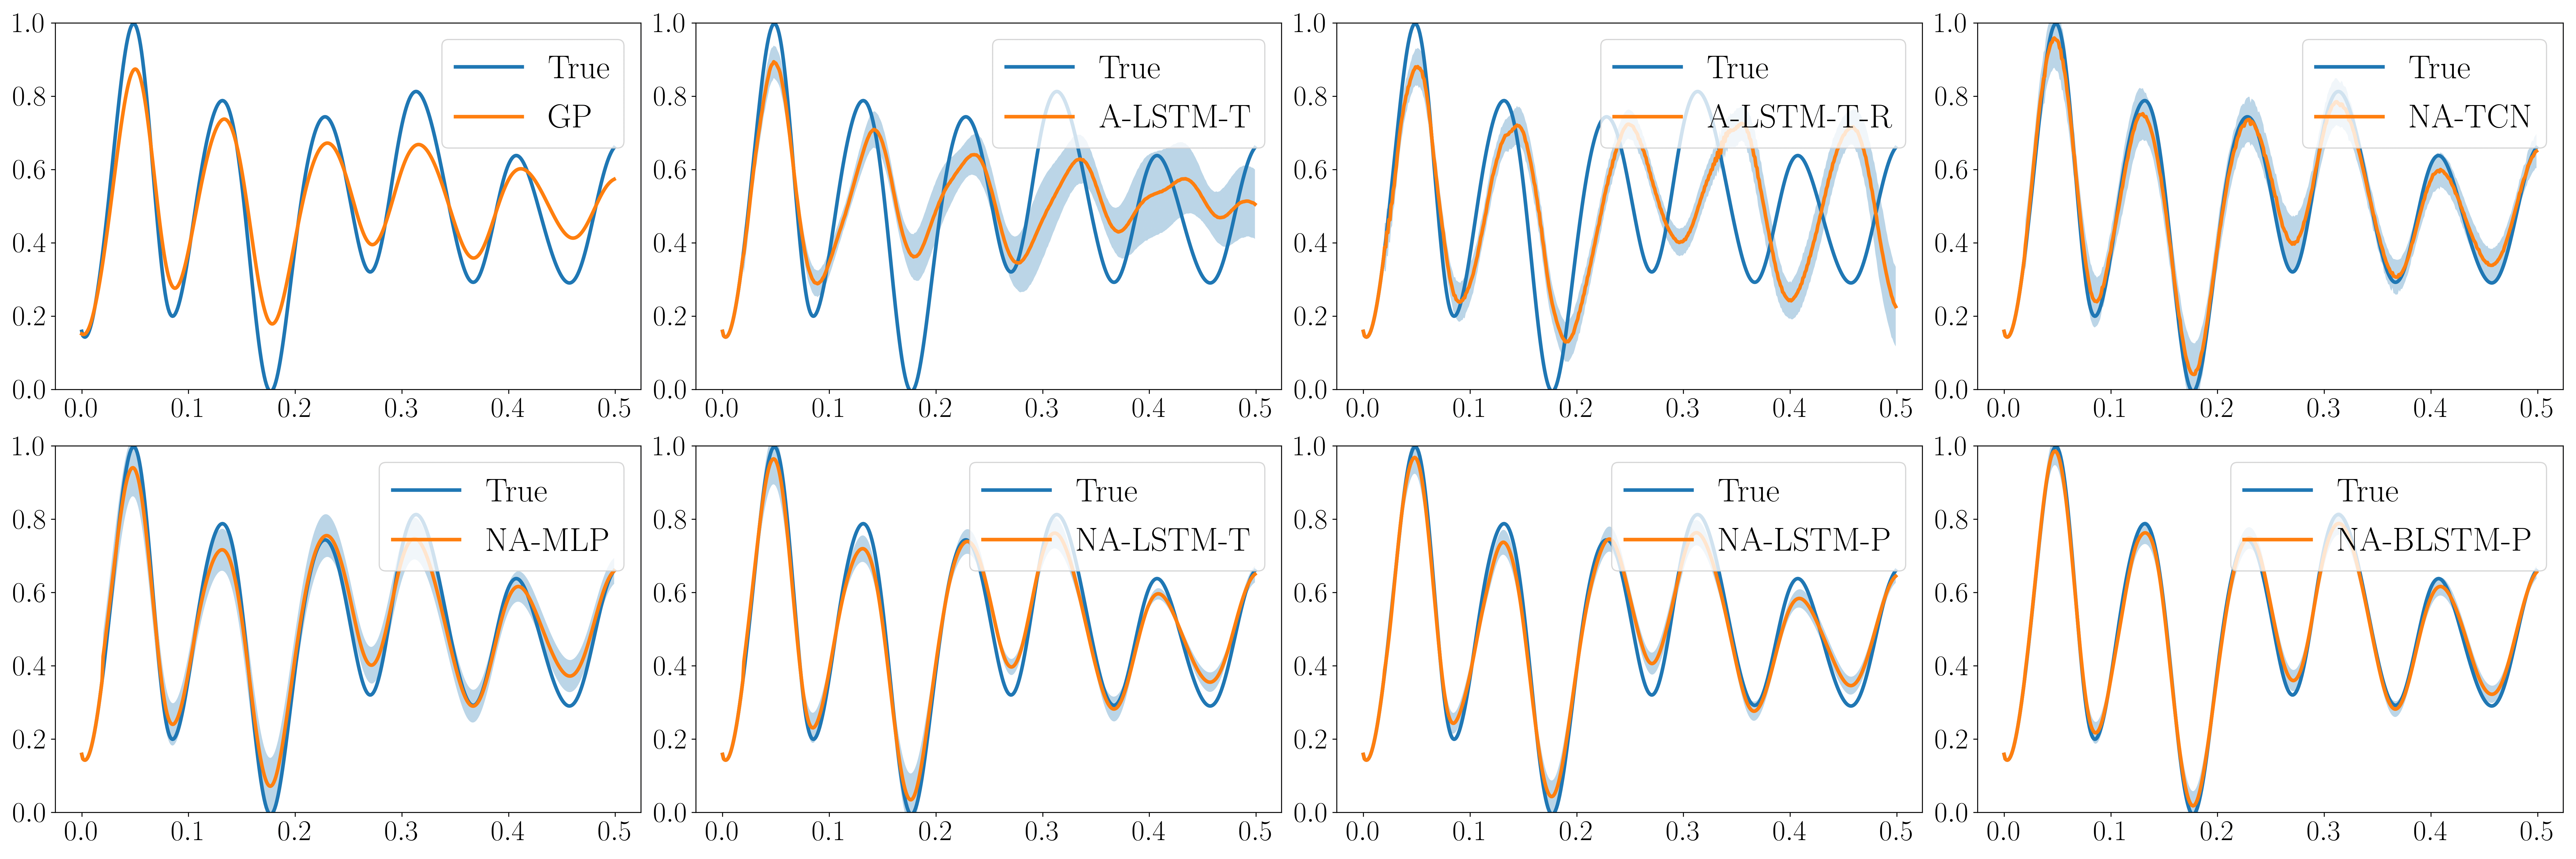
\includegraphics[width=\textwidth]{Figure_3_do.png}
    \caption{Predictive ability for the assessed frameworks for PCA component 3 with dropout at inference. We remind the reader that GP requires the solution of a partial differential equation in addition to greater observations from the true system to build a model. In addition, GP is deterministic.}
    \label{Mode_3_do}
\end{figure}

\begin{figure}[h]
    \centering
    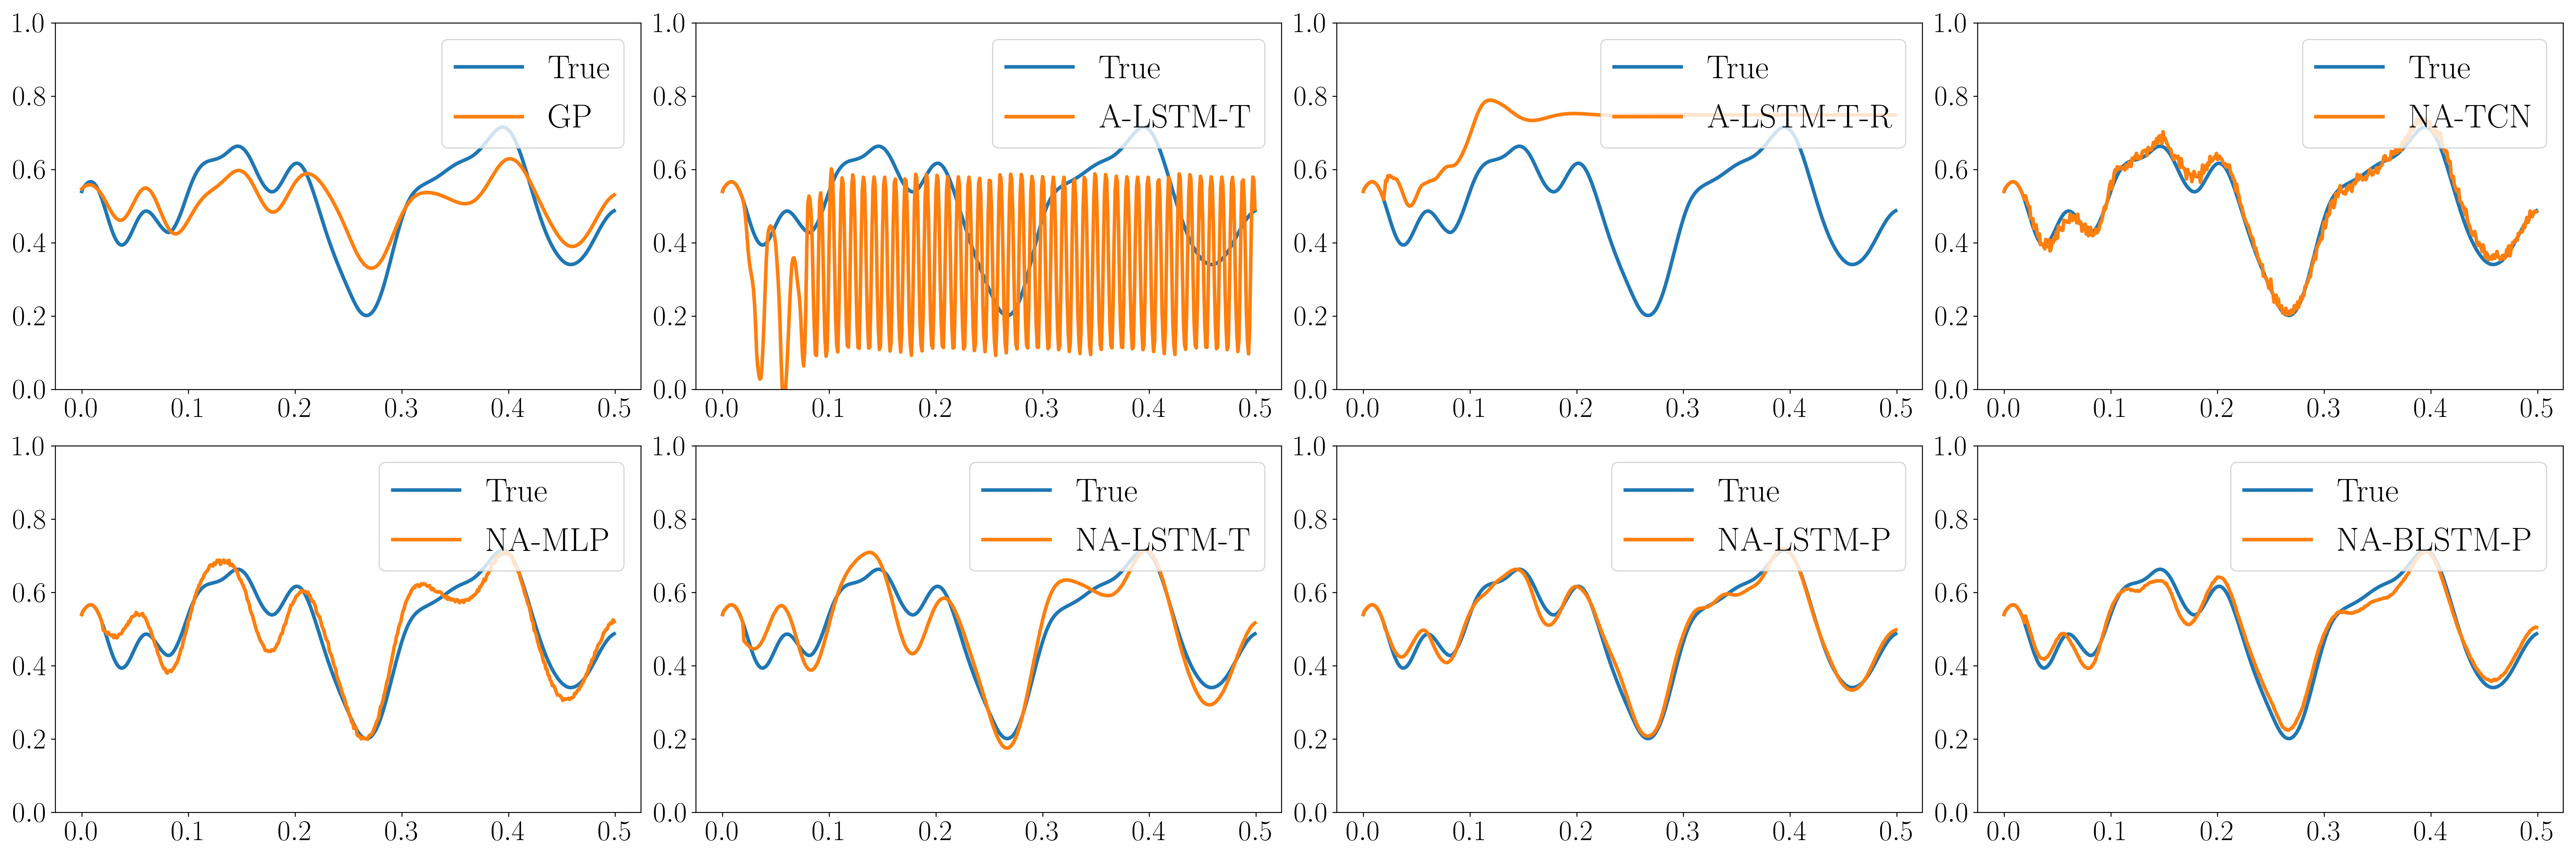
\includegraphics[width=\textwidth]{Figure_4.png}
    \caption{Predictive ability for the assessed frameworks for PCA component 4. We remind the reader that GP requires the solution of a partial differential equation in addition to greater observations from the true system to build a model. In addition, GP is deterministic.}
    \label{Mode_4}
\end{figure}

\begin{figure}[h]
    \centering
    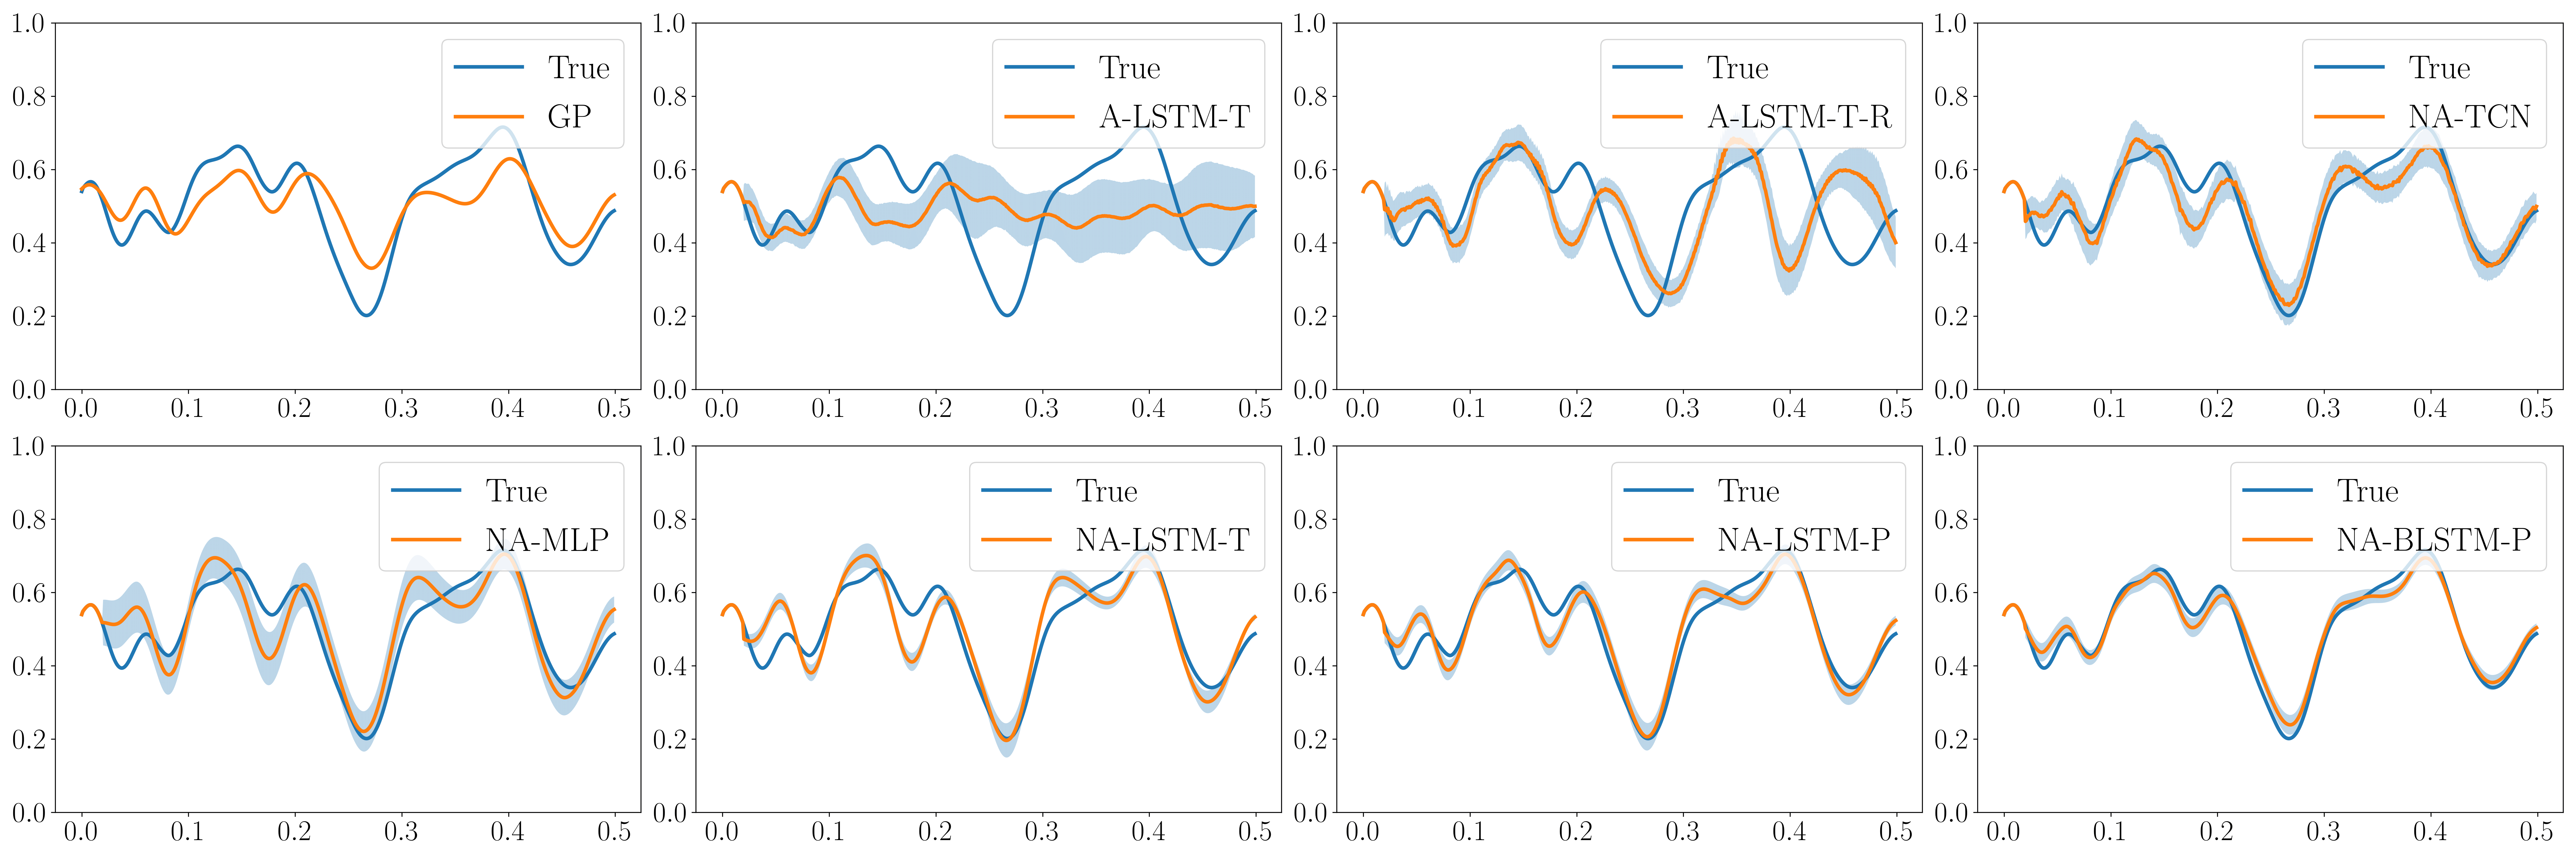
\includegraphics[width=\textwidth]{Figure_4_do.png}
    \caption{Predictive ability for the assessed frameworks for PCA component 4 with dropout at inference. We remind the reader that GP requires the solution of a partial differential equation in addition to greater observations from the true system to build a model. In addition, GP is deterministic.}
    \label{Mode_4_do}
\end{figure}

\section{Reconstruction accuracy visualized}

We plot final time fields of $\rho \eta$ in Figure \ref{Fields} using the networks obtained from Section 4.3 in the main article. Field reconstructions, compared to the truth, show that final time predictions of non-autoregressive frameworks are more successful in stable predictions.

\begin{figure}[h]
    \centering
    \includegraphics[width=\textwidth]{Fields.png}
    \caption{Predicted fields at final time. We remind the reader that GP requires the solution of a partial differential equation in addition to greater observations from the true system to build a model.}
    \label{Fields}
\end{figure}

\small
\bibliographystyle{unsrt}
\bibliography{references}

\end{document}\grid
